\chapter{Analýza metod detekce příjmu karbohydrátů}
\label{ch:analyzaCHO}
\addtocontents{toc}{\protect\setcounter{tocdepth}{1}}

Detekce příjmu karbohydrátů je důležitou součástí autonomních systémů CGMS a inzulinové pumpy. Při příjmu karbohydrátů se zvyšuje koncentrace glukózy v krvi, kterou je nutno korigovat bolusem inzulinu, aby se předešlo stavu hyperglykémie. Tato dávka inzulinu musí odpovídat množství přijatých karbohydrátů. Příliš velká dávka může vést k hypoglykémii.

Metody detekce karbohydrátů mohou být model-based nebo data-driven.

Většina studií je založená na implementaci fyzického modelu (většinou Bergmanův minimální model) a aplikaci predikčního algoritmu, jako je například Kalmanův filtr pro predikci jednotlivých stavů (glykémie a karbohydráty). Detekce karbohydrátů je pak porovnáním pozorovaných stavů a modelu vůči definovanému thresholdu, výpočtu cross-covariance nebo aplikováním rozhodovacích pravidel.

U data-driven metod se vychází z naměřených dat. Extrakce vlastností je u těchto metod kvantitativní nebo kvalitativní. Kvantitativní metoda je například analýza hlavních komponent. V kvalitativních modelech jsou časová data převedena na sekvenci kvalitativních proměnných k vytvoření kvalitativní reprezentace dat. Data-driven metody jsou méně závislé na přesnosti fyzického modelu, ale je potřeba pro jejich natrénování velkého množství vzorků. Mezi data-driven metody patří i neuronové sítě.

\section{Bergmanův minimální model}

Bergmanův minimální model \citep{analyzaCHO.Bergman} je nelineární dynamický model koncentrace glukózy v plazmě. Tento model popisuje vývoj hladiny glukózy v plazmě na základě koncentrace a účinnosti inzulinu a přijatých karbohydrátů. Model určuje sada diferenciálních rovnic prvního řádu:

$\frac{dF(t)}{dt}=-p_{1}G(t)-p_{4}I_{eff}(t)G(t)+p_{1}G_{b}+R_{a}(t)$

$\frac{dI_{eff}(t)}{dt}=-p_{2}I_{eff}(t)+p_{3}I_{p}(t)$

\noindent kde $G_b$ je koncentrace glukózy v plazmě, $I_p$ je koncentrace inzulinu v plazmě, $I_eff$ je koncentrace efektivního inzulinu, $p_1, p_2, p_3, p_4$ jsou parametry a $R_a (t)$ je míra výskytu glukózy definovaná jako:

\scalebox{1.2}{$R_{a}(t)=\frac{C(t)}{V\tau^{2}}te^{-\frac{t}{\tau}}$}

\noindent kde $C(t)$ je množství přijatých karbohydrátů, $V$  je distribuční objem a $\tau$ je vrchol absorbce karbohydrátů \citep{analyzaCHO.Turksoy}.


\section{Model-based metody}
\subsection{Real-time insulin bolusing for unannounced meals with artificial pancreas}
\label{ch:analyzaCHO:turksoy}

Pro detekční algoritmus této metody použili \citet{analyzaCHO.Turksoy} upravený Bergmanův minimální model. Unscented Kalmanův filtr je použit pro odhad stavů a parametrů minimálního modelu.

Model definuje rychlost výskytu glukózy \textbf{Ra(t)} na základě množství přijatých karbohydrátů C(t), distribučního objemu V a maximální doby absorbce jídla \textit{tau}:

\scalebox{1.2}{$R_{a}(t)=\frac{C(t)}{V\tau^{2}}te^{-\frac{t}{\tau}}$}

Rychlost výskytu glukózy \textbf{Ra(t)} je použita pro výpočet příjmu karbohydrátů. Bolus karbohydrátů je detekován pokud Ra(t) je větší než 2 mg/dl/min a naměřená hodnota z CGM je větší než 100mg/dl. Další příjem karbohydrátů může být detekován až když Ra(t) klesne pod hranici 2 mg/dl/min a uplyne alespoň 30 minut od posledního bolusu.

Testování bylo provedeno na sedmi reálných pacientech, kdy v první části experimentu si pacient aplikoval inzulin sám na základě doporučení diabetologa a ve druhé části bylo dávkování inzulinu řízeno algoritmem pro detekci karbohydrátů. Nutno podotknout, že experimentu se zúčastnili mladí lidé s optimálním glykemickým profilem. Experiment ukázal, že výsledky jsou statisticky ekvivaletní.


\subsection{Unannounced Meals in the Artificial Pancreas: Detection Using Continuous Glucose Monitoring}
\label{ch:analyzaCHO:CrossCovariance}

Autoři \citet{analyzaCHO.CrossCovariance} počítají cross-covarianci mezi naměřenými hodnotami glukózy a jejich odhadem dopředného rozdílu chybového parametru $D_{diff}$ (Unscended Kalman filter) přes tři posuvná časová okna. Pro každé okno je aplikován jiný threshold pro detekci, přičemž se snižuje riziko falešně pozitivní detekce.

\begin{figure}[H]
\caption{Naměřené hodnoty glukózy (graf 1), cross-covariance (graf 2), $D_{diff}$ parameter (graf 3)}
\label{fig:analyza:crosscovariance1}
\centering
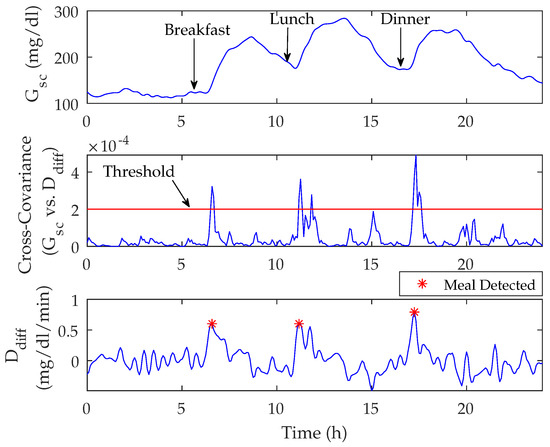
\includegraphics[width=0.8\textwidth]{img/analyzaCHO/crosscovariance1.jpg}\\
\textit{Zdroj: Unannounced Meals in the Artificial Pancreas: Detection Using Continuous Glucose Monitoring \citep{analyzaCHO.CrossCovariance}}
\end{figure}

První okno mělo vysokou míru pravdivě pozitivních detekcí, ale také falešně pozitivních. Druhé a třetí okno razantně snižuje množství falešně pozitivních detekcí, ale také se sníží množství detekovaných jídel. Zpoždění detekce bylo v průměru 30 minut u prvního okna, s každým dalším oknem se zpoždění zvyšuje.


\subsection{Probabilistic Evolving Meal Detection and Estimation of Meal Total Glucose Appearance}
\label{ch:analyzaCHO:diff}

V této práci \citet{analyzaCHO.Diff} použili inzulino-glukózový model, který udává rychlost změny intersticiální glukózy závislé na působení inzulínu a endogenní produkci glukózy. Provede se analýza změn rozdílů mezi modelovanou rychlostí změny intersticiální glukózy a naměřenou CGM. Následně jsou navzorkovány experimentálně zjištěná data příjmu karbohydrátů od 0~g do 100~g (10 vzorků) a na základě pravděpodobnosti se určí nejlepší odhad.

Na obrázku \ref{fig:analyza:diff1} je znázorněn provedený experiment při příjmu 0,33~g a 69~g karbohydrátů. První graf znázorňuje rozdíl mezi předpokládanou modelovou hodnotou glukózy a naměřenou hodnotou. Prostřední graf ukazuje pravděpodobnost příjmu karbohydrátů. Spodní graf ukazuje odhadovaný celkový výskyt glukózy z přijatého jídla. Hranice pro detekci je pravděpodobnost 10 \%.

\begin{figure}[H]
\caption{Detekce karbohydrátů v čase}
\label{fig:analyza:diff1}
\centering
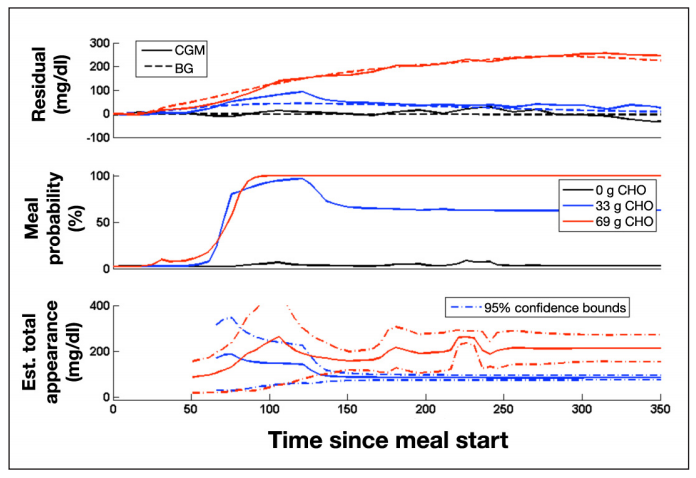
\includegraphics[width=0.7\textwidth]{img/analyzaCHO/diff1.png}\\
\textit{Zdroj: Probabilistic Evolving Meal Detection and Estimation of Meal Total Glucose Appearance \citep{analyzaCHO.Diff}}
\end{figure}

Experiment byl proveden pro 99 scénářů. Pro 11 scénářů bez jídla nebyly žádné falešně pozitivní detekce. Pro scénáře, kdy byly přijaté karbohydráty, byl algoritmus úspěšnější při příjmu většího množství karbohydrátů.


\subsection{An Unannounced Meal Detection Module for Artificial Pancreas Control Systems}
\label{ch:analyzaCHO:nekonzistence}

\citet{analyzaCHO.Nekonzistence} navrhli metodu, která využívá lineárního Kalmanova filtru nad linearizovaným Bergmanovým modelem. Přijaté karbohydráty pak způsobují nekonzistentnost tohoto filtru. Jak je v práci podotknuto, lineární Kalmanův filtr není pro tuto úlohu ideální vzhledem k tomu, že glykoregulační systém diabetického pacienta je nelineární a hladina glukózy může během dne kolísat i bez zjevných příčin. Proto se v jiných pracích používá nelineární Unscented Kalmanův filtr. Úspěšnost a rychlost detekce pro různou velikost jídel je vidět v tabulce na obrázku \ref{fig:analyza:nekonzistence}.

\begin{figure}[H]
\caption{Úspěšnost detekce vzhledem hladině glukózy a množství přijatých karbohydrátů}
\label{fig:analyza:nekonzistence}
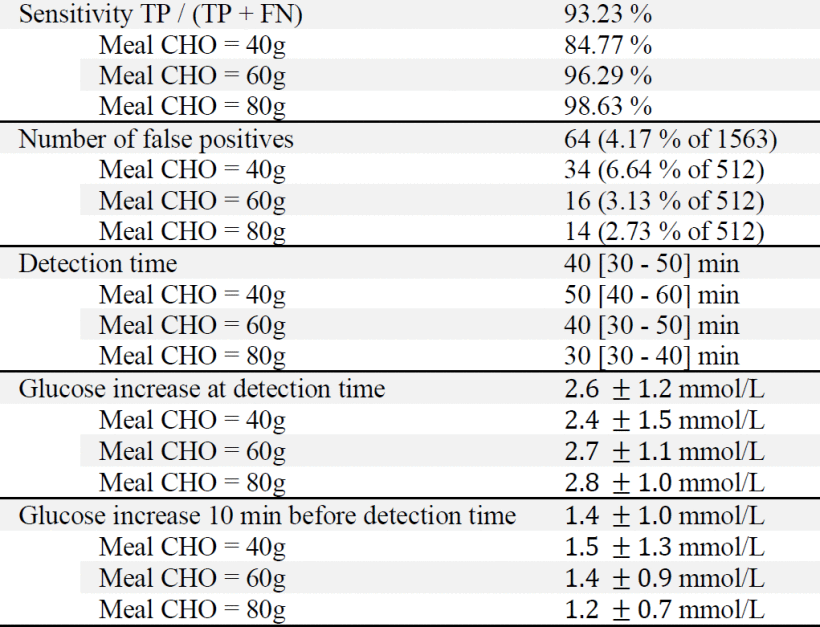
\includegraphics[width=0.8\textwidth]{img/analyzaCHO/nekonzistence.png}\\
\textit{Zdroj: An Unannounced Meal Detection Module for Artificial Pancreas Control Systems \citep{analyzaCHO.Nekonzistence}}
\end{figure}


\subsection{Committed Moving Horizon Estimation for Meal Detection and Estimation in Type 1 Diabetes}
\label{ch:analyzaCHO:horizon}

Committed Moving Horizon Estimation (CMHE) \citep{analyzaCHO.MovingHorizon} umožňuje predikovat čas a velikost nehlášených jídel. Metoda je založena na Moving Horizon Estimation (MHE). MHE je metoda odhadů omezených stavů nelineárního diskrétního modelu, která predikuje sekvenci stavových proměnných a poruch $\delta$ (disturbance) tak, že minimalizuje chybu mezi predikovanými a měřenými hodnotami \citep{analyzaCHO.MovingHorizon}. V případě detekce karbohydrátů je modelem glukózo regulační systém člověka (ve studii je použit Bergmanův minimální model) a poruchami se rozumí přijaté karbohydráty. MHE, na rozdíl od Kalmanova filtru, nepočítá s normálním rozdělením poruch. 

Pro každou instanci MHE (časové okno velikosti N) je N odhadů disturbance hodnoty (pro t až t-N). V každém časovém bodě t tak máme N odhadů v čase t+N. Problémem je, který z N odhadů vybrat. Prvotní odhad v čase t není přesný, protože tento odhad zohledňuje pouze naměřené hodnoty před časem t, zatímco zvýšení hladiny glukózy se projeví až s časovým odstupem od přijetí karbohydrátů v závislosti na metabolismu daného člověka. Odhad v čase t+N zase nezohledňuje vývoj glukózy v minulosti a zároveň je k dispozici s velkým zpožděním. Tento problém řeší CMHE, který nebere jednu disturbance hodnotu, ale kompromis mezi predikovanými a naměřenými hodnotami. Výsledná hodnota disturbance parametru v čase $\Delta_{t-V}$ je vypočítá jako vážený průměr odhadů v daný čas z předchozích iterací včetně (obrázek \ref{fig:analyza:horizon1}):

\scalebox{1.5}{$\Delta_{t-V}=\frac{(\sum^{t}_{i=t-V+1}W(i)^{b}\cdot \delta^{i}_{t-V})}{\sum^{t}_{i=t-V+1}W(i)^{b}}$}

kdy V je commitment level, V<N, $\delta$ je disturbance parametr, W(i) jsou váhy prioritizující odhady mezi predikovanými a naměřenými hodnotami.

\begin{figure}[H]
\caption{Disturbance paremetr $\delta$ několik časových oken}
\label{fig:analyza:horizon1}
\centering
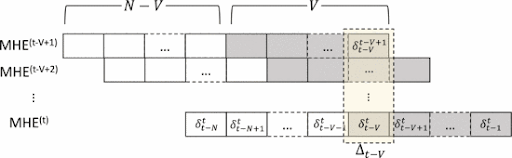
\includegraphics[width=1\textwidth]{img/analyzaCHO/horizon1.png}\\
\textit{Zdroj: Committed Moving Horizon Estimation for Meal Detection and Estimation in Type 1 Diabetes \citep{analyzaCHO.MovingHorizon}}
\end{figure}

CMHE instance (min Ct) se optimalizují pomocí Mixed-integer Quadratic Programming (MIQP), který disturbance parametr reprezentuje jako čtvercovou vlnu (za předpokladu, že příjem karbohydrátů po dobu jídla je konstantní). Jídlo je detekováno pokud $\Delta t$ je nad daným thresholdem alespoň 80 \% času w.

V provedeném experimentu je měření prováděno každou minutu, časové okno N = 180, commitment level V = 40, w = 5 minut. Na obrázku \ref{fig:analyza:horizon4} je srovnání MHE a CMHE v závislosti na nastaveném thresholdu.  V tabulce \ref{tab:analyza:horizon5} jsou výsledky experimentu pro jednotlivá jídla, kdy nastavený threshold je optimální (černý trojúhelník). Metoda dosahuje 100 \% úspěšnost detekce pro hlavní jídla, celkových 88.5 \% je způsobeno menšími jídly, pro jejichž lepší detekci by musel být snížen threshold. To by ale vedlo ke zvýšení falešných detekcí, kterých je v průměru 2.6 za den. Průměrná doba detekce je 20 minut \citep{analyzaCHO.MovingHorizon}.

\begin{figure}[H]
\caption{Detekce MHE (modrá) a CMHE (červená)}
\label{fig:analyza:horizon4}
\centering
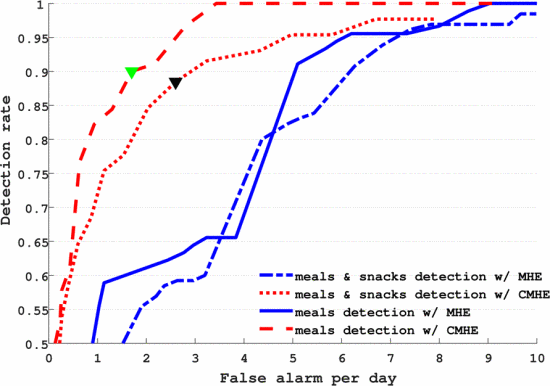
\includegraphics[width=0.9\textwidth]{img/analyzaCHO/horizon4.png}\\
\textit{Zdroj: Committed Moving Horizon Estimation for Meal Detection and Estimation in Type 1 Diabetes \citep{analyzaCHO.MovingHorizon}}
\end{figure}

\begin{table}[H]
\caption{Výsledky}
\label{tab:analyza:horizon5}
\centering
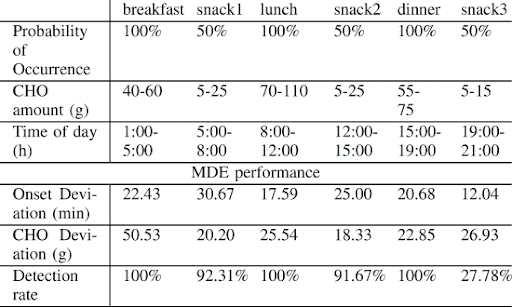
\includegraphics[width=0.8\textwidth]{img/analyzaCHO/horizon5.png}\\
\textit{Zdroj: Committed Moving Horizon Estimation for Meal Detection and Estimation in Type 1 Diabetes \citep{analyzaCHO.MovingHorizon}}
\end{table}


\section{Data-driven metody}
\subsection{Unannounced Meal Detection for Artificial Pancreas Systems Using Extended Isolation Forest}
\label{ch:analyzaCHO:forest}

Isolation forest je metoda, která detekuje a izoluje anomálie v datech. Data jsou rekurzivně rozdělena do stromové struktury (iTree - isolation tree) náhodným výběrem atributů z daných vlastností (feature) dokud nejsou jednotlivé instance izolovány. Toto náhodné rozdělení má pro anomálie signifikantně kratší cestu ve stromové struktuře \citep{analyzaCHO.IsolationForest}.

Vlastnosti, které slouží jako vstup pro Extended isolation forest \citep{analyzaCHO.ExtendedIsolationForest} jsou derivace naměřené glukózy v plazmě \textbf{dGp}, zadané karbohydráty (pokud byly zadány) a podaný inzulin. Pro výpočet derivace glukózy v čase t \textbf{dGp(t)} je potřeba znát naměřenou glukózu v čase t+1 \textbf{Gp(t+1)}. Z toho důvodu nastává zpoždění detekce o 5 minut. Detekce anomálií je pak pomocí dvou thresholdů pro menší a větší míru rizika nezadaných karbohydrátů.
Příklad detekce anomálií je na obrázku \ref{fig:analyza:forest}. Notifikace je vznešena pokud se objeví jedna anomálie s větší mírou rizika (červené), nebo 3 anomálie s menší mírou rizika (modré).

\begin{figure}[H]
\caption{Úspěšnost detekce vzhledem hladině glukózy a množství přijatých karbohydrátů}
\label{fig:analyza:forest}
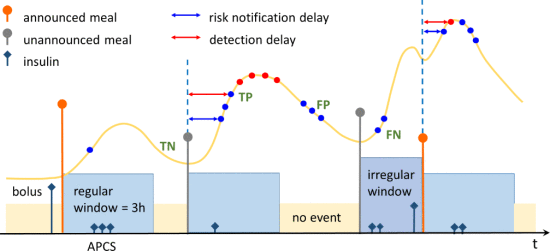
\includegraphics[width=1\textwidth]{img/analyzaCHO/forest.png}\\
\textit{Zdroj: Unannounced Meal Detection for Artificial Pancreas Systems Using Extended Isolation Forest \citep{analyzaCHO.ExtendedIsolationForest}}
\end{figure}

Metoda byla testována na čtyřech virtuálních pacientech (pro jejich simulaci byl využit Hovorkovo model) V simulovaných pětidenních denních scénářích přijal pacient průměrně 3,4 jídla za den. Pro scénář, kdy bylo jídlo v 50 \% zadáno a v 50 \% nezadáno, dosahovala metoda úspěšnosti 90,8 \% a v 6,2 \% případů byla falešně pozitivní. V případě, že jídlo nebylo zadáno vůbec, byla úspěšnost 90,0 \% a v 11,47 \% falešně pozitivní. Zpoždění detekce je 26-39 minut \citep{analyzaCHO.ExtendedIsolationForest}.


\subsection{A Closed-Loop Artificial Pancreas Using Model Predictive Control and a Sliding Meal Size Estimator}
\label{ch:analyzaCHO:thrashold}

\citet{analyzaCHO.Thresholds} použili hlasovací schéma pro detekci karbohydrátů. Algoritmus je založen na kontinuálním  pozorování první a druhé derivace koncentrace glukózy, které při splnění kritérii vyšle sérii impulsů (až 15 impulsů během 30ti minut). Tato metoda je založena na vzorkování po jedné minutě.

Impulsy jsou vyslány při překročení thresholdu. Pro nastavení thresholdu se vychází z toho, že jedno jídlo způsobí nárůst rychlosti výskytu glukózy v krvi $dG$ (první derivace) 0-2 mg/dl/min, druhé derivace $d_{2}G$ 0-0,02 mg/dl/min2. Thresholdy jsou proto nastaveny na {0, 0.5, 1.25, 1.8} pro $dG$ a {0, 0.005, 0.0125, 0.018} pro $d_{2}G$. Jelikož je mezi $dG$ a $d_{2}G$ zpoždění, další impuls je vyslán pokud se hodnoty kříží. Vyslání impulsů je na obrázku \ref{fig:analyza:threshold1}.
 
Tyto impulsy jsou poté zesíleny a převedeny na gramy karbohydrátů (ve studii počítají se 4~g na impuls), viz obrázek \ref{fig:analyza:threshold2}.

Počet impulsů, časové okno, thresholdy a množství karbohydrátů na impuls lze individuálně změnit podle diabetického profilu pacienta.

\begin{figure}[H]
\caption{Impulsy}
\label{fig:analyza:threshold1}
\centering
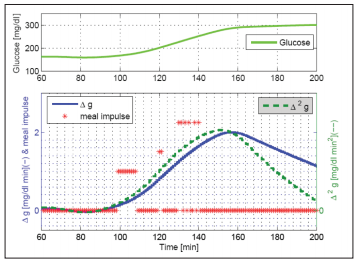
\includegraphics[width=0.8\textwidth]{img/analyzaCHO/threshold1.png}\\
\textit{Zdroj: A Closed-Loop Artificial Pancreas Using Model Predictive Control and a Sliding Meal Size Estimator \citep{analyzaCHO.Thresholds}}
\end{figure}
\begin{figure}[H]
\caption{Predikované karbohydráty}
\label{fig:analyza:threshold2}
\centering
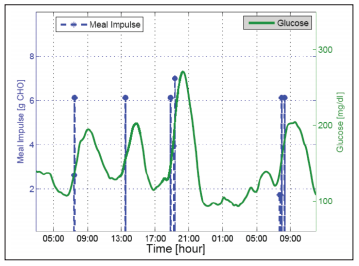
\includegraphics[width=0.8\textwidth]{img/analyzaCHO/threshold2.png}\\
\textit{Zdroj: A Closed-Loop Artificial Pancreas Using Model Predictive Control and a Sliding Meal Size Estimator \citep{analyzaCHO.Thresholds}}
\end{figure}

Algoritmus detekuje 656 jídel z 800 (82 \%) a 144 falešně pozitivních detekcí. Průměrný odhad jídla je 36,41~g karbohydrátů. Zpoždění detekce je průměrně 31 minut \citep{analyzaCHO.Thresholds}.


\subsection{Meal Detection and Carbohydrate Estimation Using Continuous Glucose Sensor Data}
\label{ch:analyzaCHO:wavelet}

V této studii \citet{analyzaCHO.WaveletEst} použili waveletové filtrování pro odstranění šumu z dat naměřených CGM. Waveletové filtrování rozdělí frekvenční obsah vstupních dat do několika pásem, kde se jinou měrou projevuje šum a užitečná složka \citep{analyzaCHO.Wavelet}. Zvolený parametr míry filtrování musí být dostatečně velký, aby odfiltroval šum, ale ne přiliš, aby se neodfiltrovaly ostré nárůsty způsobené příjmem karbohydrátů.

Pro extrakci vlastností je použita trojúhelníková kvalitativní reprezentace. V kvalitativních metodách extrakce dat jsou časová data konvertována na sekvenci kvalitativních proměnných. Pro trojúhelníkovou kvalitativní reprezentaci jsou kvalitativní proměnné trojúhelníky (viz obrázek \ref{fig:analyza:wavelet1}). Trojúhelníky dělí data na epizody (obrázek \ref{fig:analyza:wavelet2}) jejichž hraniční body jsou buďto extrém ($dG/dt=0$) nebo inflexní bod ($d_{2}G/dt=0$). Epizody se nepřekrývají a každé dvě sousední jsou rozdílné. Hodnoty dx a ddx jsou vypočteny z numerické derivace a mapovány na +/0/-.

\begin{figure}[H]
\caption{Kvalitativní proměnné trojúhelníkové kvalitativní reprezentace}
\label{fig:analyza:wavelet1}
\centering
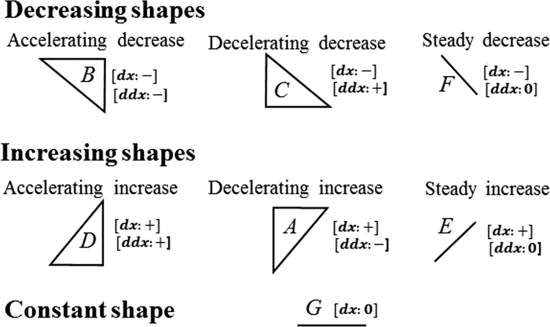
\includegraphics[width=0.6\textwidth]{img/analyzaCHO/wavelet1.png}\\
\textit{Zdroj: Meal Detection and Carbohydrate Estimation Using Continuous Glucose Sensor Data \citep{analyzaCHO.WaveletEst}}
\end{figure}
\begin{figure}[H]
\caption{Data rozdělená na epizody}
\label{fig:analyza:wavelet2}
\centering
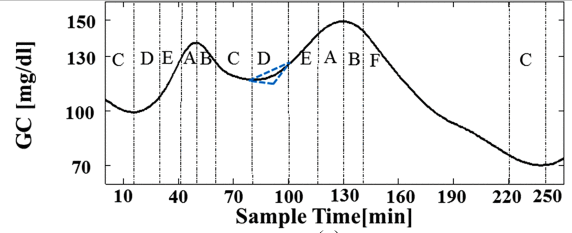
\includegraphics[width=0.8\textwidth]{img/analyzaCHO/wavelet2.png}\\
\textit{Zdroj: Meal Detection and Carbohydrate Estimation Using Continuous Glucose Sensor Data \citep{analyzaCHO.WaveletEst}}
\end{figure}

Pro tuto studii byla definice epizod modifikována tak, že velikost epizody je pevně dána a obsahuje určitý počet vzorků. Epizody se překrývají a sousední mohou být stejné. Výpočet dx a ddx udávající tvar trojúhelníku je:

$d^{1}G(n)=G(n)-G(n-l_{e})$

$d^{2}G(n)=G'(n)-G'(n-l_{e})$

$G'(n)=G(n)-G(n-1)$

Do trojúhelníkové reprezentace se přidá neurčitost (fuzzy logika) tak, že epizodu popisuje více tvarů trojúhelníků (definují se další způsoby pro výpočet $d^1x$ a $d^2x$).

Pro detekci příjmu karbohydrátů se každému trojúhelníku přiřadí váha odpovídající tvaru. Vynásobením vah s vektorem fuzzy trojúhelníkové reprezentace vznikne proměnná \textit{“increase of glucose trend index”} Igt pro každý vzorek (váhy jsou nastaveny tak, že hodnota $I_gt$ je v intervalu<-3;3>). Pakliže hodnota Igt (nebo součet Igt v časovém okně) překročí hranici 2,5, je detekován příjem.

Úspěšnost detekce byla u dospělých 87 \% (falešně pozitivní 21 \%) a u dětí 93 \% (falešně pozitivní 3 \%). Zpoždění detekce je přibližně půl hodiny \citep{analyzaCHO.WaveletEst}.


\subsection{Pattern Recognition Reveals Characteristic Postprandial Glucose Changes: Non-Individualized Meal Detection in Diabetes Mellitus Type 1}
\label{ch:analyzaCHO:lda}

\citet{analyzaCHO.LDA} použili Moving horizon estimator pro odhad glukózy a lineární diskriminační analýzu pro klasifikaci.

Porovnávány jsou 4 metody (2 na základě klasifikace a 2 metody pro porovnání za použití thresholdu):

\begin{enumerate}
\item \textbf{Klasifikace odhadu Ra horizontů} \\
Odhady rychlosti výskytu glukózy Ra horizontů jsou predikovány na základě Bergmanova modelu. Na tyto Ra je použita Lineární diskriminační analýza (LDA).
\item \textbf{Klasifikace CGM horizontů} \\
Klasifikace je na hrubých vyhlazených datech z CGM modulu. Také v tomto případě je použita LDA.
\item \textbf{Threshold pro aktuální Ra odha} \\
Detekce přijatých karbohydrátů je pokud Ra překročí daný threshold (viz kapitola \ref{ch:analyzaCHO:turksoy}).
\item \textbf{GRID algoritmus} \\
Threshold pro naměřené hodnoty glukózy a jejich rychlost změny.
\end{enumerate}

Na obrázku \ref{fig:analyza:lda1} je výkonnost jednotlivých metod při provedeném experimentu. Je vidět, že metody využívající LDA si vedly výrazně lépe. Jejich úspěšnost se pohybuje kolem 88 \%. Také v případě času potřebného k detekci překonaly metody založené na thresholdu. Srovnání zpoždění u jednotlivých metod je na obrázku \ref{fig:analyza:lda2}.

\begin{figure}[H]
\begin{minipage}{.5\textwidth}
\caption{Úspěšnost detekce}
\label{fig:analyza:lda1}
\centering
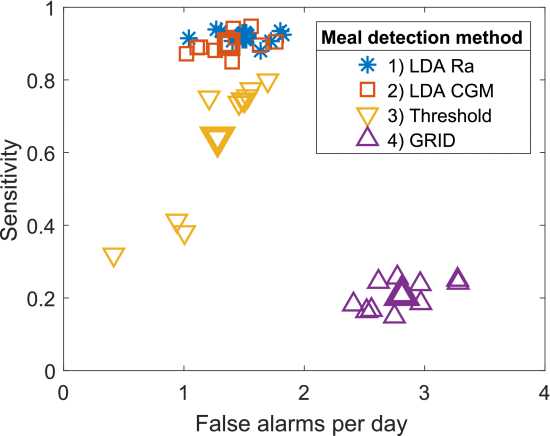
\includegraphics[width=1\textwidth]{img/analyzaCHO/lda1.png}\\
\end{minipage}
\begin{minipage}{.5\textwidth}
\caption{Zpoždění detekce}
\label{fig:analyza:lda2}
\centering
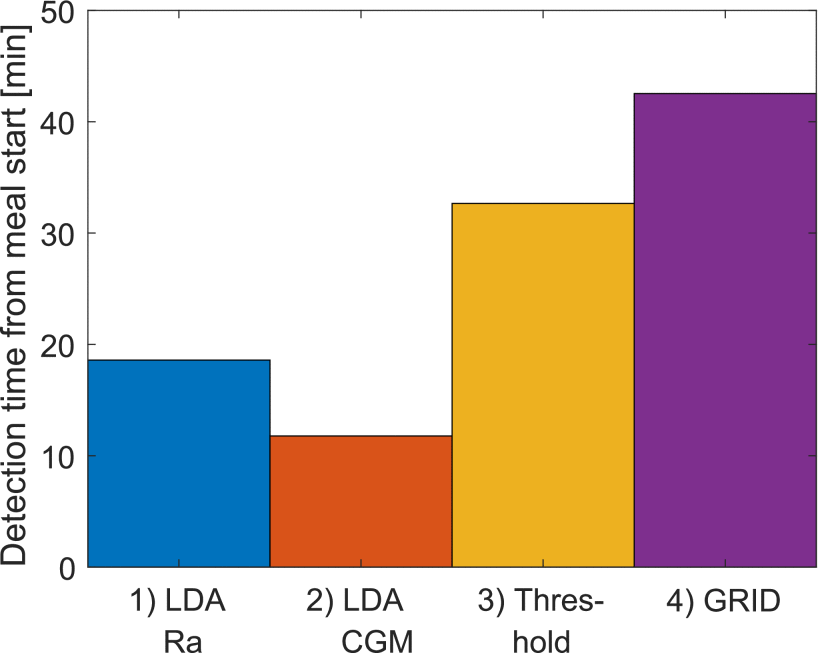
\includegraphics[width=1\textwidth]{img/analyzaCHO/lda2.png}\\
\end{minipage}
\textit{Zdroj: Pattern Recognition Reveals Characteristic Postprandial Glucose Changes: Non-Individualized Meal Detection in Diabetes Mellitus Type 1 \citep{analyzaCHO.LDA}}
\end{figure}


\section{Metody využívající neuronové sítě}
\subsection{Predicting the meal macronutrient composition from continuous glucose monitors}
\label{ch:analyzaCHO:neuronka}

V této studii \citet{analyzaCHO.Neuronka} použili multitaskovou neurální síť pro určení složení (karbohydráty, proteiny, tuky) v přijatém jídle.

Pro zachycení charakteristických vlastností z dat CGM byl vypočten určitý integrál (oblast pod křivkou) pro 5 časových bodů (klidový stav nalačno, zvýšená glykémie, střední hodnota při návratu do klidového stavu, pokles glukózy a konečný stav).

Multitasková neuronová síť obsahuje jednu společnou vrstvu pro vstup (vypočítané integrály) a výstupní vrstvu (viz obrázek \ref{fig:analyza:neuronka}). Aktivační funkce pro vstupní vrstvu je Rectified Linear Units (ReLU), pro výstupní lineární funkce, ztrátová funkce je Huberova ztrátová funkce. Trénování neuronové sítě bylo na 1000 epochách.

\begin{figure}[H]
\caption{Neuronová síť}
\label{fig:analyza:neuronka}
\centering
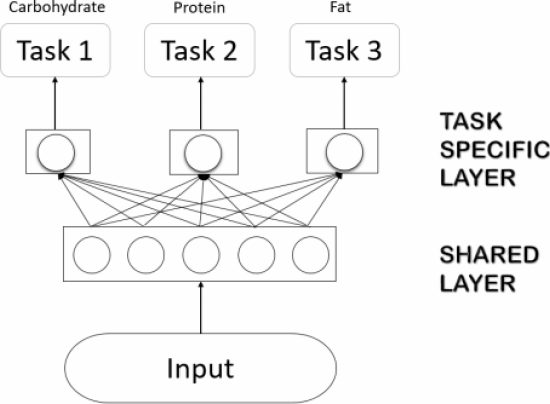
\includegraphics[width=0.7\textwidth]{img/analyzaCHO/neuronka.png}\\
\textit{Zdroj: Predicting the meal macronutrient composition from continuous glucose monitors \citep{analyzaCHO.Neuronka}}
\end{figure}

Trénování neuronové sítě a následná cross-validace byla provedena pro dva scénáře. První je natrénování neuronové sítě na datech několika pacientů a validace na datech jiného pacienta. Druhý způsob spočívá v natrénování neuronové sítě na části dat jediného pacienta (vynechání jednoho jídla) a validace na zbylých datech. Z experimentu vyšel lépe druhý způsob zohledňující metabolismus konkrétního jedince se střední kvadratickou chybou pro karbohydráty 0,39. Kvadratická chyba karbohydrátů pro první způsob je 0,45 \citep{analyzaCHO.Neuronka}. 

Metoda počítá s poměrně přesným příjmem jídla v časovém rozmezí 8 hodin. Jako vstup pro neuronovou síť pak jsou vypočtená data z tohoto celého časového okna. Při sběru dat byla také vyloučená fyzická aktivita, která ovlivňuje hladinu glukózy. Z těchto důvodů není metoda vhodná pro řízení dávkování inzulinu v reálném čase.


\subsection{Continuous glucose monitoring prediction}

V této studii \citet{analyzaCHO.LSTM} implementovali 3 různé algoritmy pro vývoj glykémie po jídle. Studie se nezabývá vlastní detekcí příjmu karbohydrátů.

Seasonal Autoregressive Integrated Moving Average (SARIMA) je regresní model pro časové řady. SARIMA počítá s trendem a sezónními parametry, které musí být před použitím nastaveny. Pro nastavení těchto parametrů byla použita autokorelace a částečná autokorelace.

V druhé metodě je použit Kalmanův filtr pro predikci vývoje hladiny glukózy pacienta.

V poslední metodě jsou implementovány dvě rekurentní neuronové sítě, konkrétně Long Short Term Memory model (LSMT). Pro druhou neuronovou síť slouží výstup LSMT jako vstup do další vrstvy spolu s konstantami. Těchto 7 konstant jsou první, druhý peak a střední hodnota Fourirovy transformace, střední hodnota a rozptyl Waveletové transformace a diskrétní Waveletové transformace provedenými nad daty CGM. Model byl natrénován na 10 epoch.

Pro výpočet chyby a ztrátové funkce u všech metod je použita střední absolutní chyba (MEA) a střední kvadratická chyba (RMSD). V tabulce \ref{tab:analyza:lstm} jsou výsledky jednotlivých metod.

\begin{table}[H]
\caption{Výsledky}
\label{tab:analyza:lstm}
\centering
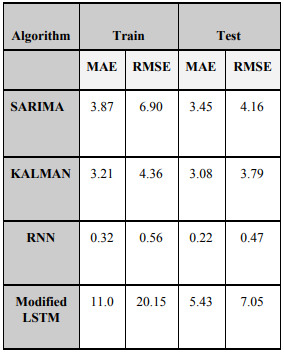
\includegraphics[width=0.5\textwidth]{img/analyzaCHO/lstm.png}\\
\textit{Zdroj: Continuous glucose monitoring prediction \citep{analyzaCHO.LSTM}}
\end{table}

\newpage

\section{Porovnání jednotlivých metod}

V tabulce \ref{tab:analyza:res} je srovnání jednotlivých metod pro detekci karbohydrátů. Kritérii pro porovnání jednotlivých metod je přesnost detekce a zpoždění detekce od doby příjmu karbohydrátů.

\begin{table}[H]
\caption{Porovnání jednotlivých metod}
\label{tab:analyza:res}
\hskip-1.0cm
\begin{tabular}{|l|l|c|c|c|c|}
\hline 
\textbf{Studie} & \textbf{Zpoždění*} & \textbf{TP} & \textbf{FN} & \textbf{TN} & \textbf{FP}\tabularnewline
\hline 
\hline 
\ref{ch:analyzaCHO:turksoy} \citet{analyzaCHO.Turksoy} & - & - & - & - & -\tabularnewline
\hline 
\ref{ch:analyzaCHO:CrossCovariance} \citet{analyzaCHO.CrossCovariance} & 25-40 & 91.6\%{**} & - & - & -\tabularnewline
\hline 
\ref{ch:analyzaCHO:diff} \citet{analyzaCHO.Diff} & - & - & - & 11 & 0\tabularnewline
\hline 
\ref{ch:analyzaCHO:nekonzistence} \citet{analyzaCHO.Nekonzistence} & 30-50 & 93.23\% & 6.77\% & - & 4.17\%\tabularnewline
\hline
\ref{ch:analyzaCHO:horizon} \citet{analyzaCHO.MovingHorizon} & 20 & 88.5\% & 11.5\% & - & 2.6FP/den\tabularnewline
\hline 
\ref{ch:analyzaCHO:forest} \citet{analyzaCHO.ExtendedIsolationForest} & 26-39 & 90\% & 10\% & - & 11.47\%\tabularnewline
\hline 
\ref{ch:analyzaCHO:thrashold} \citet{analyzaCHO.Thresholds} & 31 (avg.) & 656 (82\%) & 144 (18\%) & - & 54 (6.75\%)\tabularnewline
\hline 
\ref{ch:analyzaCHO:wavelet} \citet{analyzaCHO.WaveletEst} & 30 (avg.) & 87\% & 13\% & - & 21\%\tabularnewline
\hline 
\ref{ch:analyzaCHO:lda} Ra \citet{analyzaCHO.LDA} & 18.59 & 92\% & 8\% & - & 1.5FP/den\tabularnewline
\hline 
\ref{ch:analyzaCHO:lda} CGM \citet{analyzaCHO.LDA} & 11.78 & 90\% & 10\% & - & 1.37FP/den\tabularnewline
\hline
\ref{ch:analyzaCHO:neuronka} \citet{analyzaCHO.Neuronka} & 8 hodin & 0.39{***} & & & \tabularnewline
\hline
\end{tabular}
\begin{flushleft}
* doba detekce karbohydrátů od příjetí jídla v minutách\\
{**} úspěšnost detekce jednotlivých oken v tabulce\\
{***} RMSRE - střední kvadratická chyba\\
TP - true positive\\
TN - true negative\\
FP - false positive\\
FN - false negative\\
\end{flushleft}
\end{table}


\addtocontents{toc}{\protect\setcounter{tocdepth}{2}}